\section{Binary Trees}
In Prolog, we do not need special pointers or object classes to represent hierarchical data structures. Instead, we represent a \textbf{binary tree} inductively using compound terms:
\begin{itemize}
    \item \textbf{The empty tree} is represented by the atom \texttt{nil}.
    \item \textbf{A non-empty node} is represented by the 3-ary functor \texttt{tree(Value, Left, Right)}, where \texttt{Value} is the stored item, and \texttt{Left} and \texttt{Right} are themselves binary subtrees.
\end{itemize}
For example, a leaf node containing $1$ is written as \texttt{tree(1, nil, nil)}, while a tree with root $1$ and children $2$ and $3$ is represented as:
\[
\texttt{tree(1, tree(2, nil, nil), tree(3, nil, nil))}
\]
\minititle{Structural Validation: \texttt{is\_b\_tree/1}}
Before performing operations on trees, we want to write a recognizer predicate \texttt{is\_b\_tree(T)} that succeeds if and only if \texttt{T} is a structurally well-formed binary tree.
The inductive definition is straightforward:
\begin{itemize}
    \item \textbf{Base Case:} The empty tree \texttt{nil} is a valid binary tree.
    \item \textbf{Recursive Step:} A compound term \texttt{tree(\_, L, R)} is a valid binary tree if both its left subtree \texttt{L} and right subtree \texttt{R} are valid binary trees.
\end{itemize}
\begin{codeblock}
is_b_tree(nil).
is_b_tree(tree(_, L, R)) :-
    is_b_tree(L),
    is_b_tree(R).
\end{codeblock}
We can verify our representation:
\begin{codeblock}
?- is_b_tree(tree(1, tree(2, nil, nil), tree(3, nil, nil))).
true.
?- is_b_tree(tree(1, invalid_child, nil)).
false.
\end{codeblock}

\minititle{Count Nodes}

We want to count the nodes in a binary tree with the predicate \texttt{bt\_nodes\_count(Tree, Count)}. For the base case, the empty tree has zero nodes. For non-empty trees, the number of nodes is the number of nodes in the left sub-tree added to the number of nodes in the right sub-tree added to one (the root of the tree).

\begin{codeblock}
bt_nodes_count(nil,0):-!.
bt_nodes_count(tree(_, L, R), Res):-
    bt_nodes_count(L,LeftNodes),
    bt_nodes_count(R,RightNodes),
    Res is LeftNodes + RightNodes + 1.
\end{codeblock}

\begin{codeblock}
?- bt_nodes_count(tree(5,tree(3,nil,nil),tree(7,nil,nil)), X).
X = 3
\end{codeblock}

\minititle{Count Leaves}

\texttt{bt\_leaves\_count/2} should count only the leaves of a BT. We have two base cases:
\begin{itemize}
    \item Empty tree $\leadsto$ 0 
    \item A leaf (\texttt{tree(\_,nil,nil)}) $\leadsto$ 1 
\end{itemize}

Otherwise, the sum of the leaves count from the right and left subtrees!

\begin{codeblock}
bt_leaves_count(nil,0):-!.
bt_leaves_count(tree(_,nil,nil),1):-!.
bt_leaves_count(tree(_, L, R), Res):-
    bt_leaves_count(L,LeftLeaves),
    bt_leaves_count(R,RightLeaves),
    Res is LeftLeaves + RightLeaves.
\end{codeblock}

\begin{codeblock}
?- bt_leaves_count(tree(5,tree(3,nil,nil),tree(7,nil,nil)), X).
X = 2
\end{codeblock}

\minititle{Symmetric}
We want to write a predicate \texttt{symmetric/1} that is only true if the binary tree is symmetric. A symmetric BT would look exactly the same if it was mirrored, i.e. flipped horizontally (the subtrees \textbf{mirror} each other).

\begin{figure}[H]
    \centering
    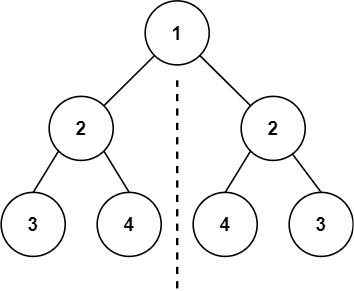
\includegraphics[width=0.3\linewidth]{images/symtree1.jpg}
\end{figure}

\ideabox{
Let's write a helper predicate \texttt{mirror/2} that checks if two BTs mirror each other!
}

The empty tree mirrors itself. For two non-empty trees, they mirror each other if their subtrees do!

\begin{codeblock}
mirror(nil,nil):-!.
mirror(tree(N,L1,R1), tree(N,L2,R2)):-
    mirror(L1,R2),
    mirror(R1,L2).
\end{codeblock}

Let's test that on the subtrees of the image above:

\begin{codeblock}
?- mirror(tree(2, tree(3, nil,nil), tree(4, nil,nil)),
       tree(2, tree(4, nil,nil), tree(3, nil,nil))).
true
\end{codeblock}

\ideabox{
Checking symmetry becomes easier now. The empty tree is symmetric. The non-empty tree is symmetric if its left subtree mirrors its right subtree!
}

\begin{codeblock}
symmetric(nil):-!.
symmetric(tree(_,L,R)):-
    mirror(L,R).
\end{codeblock}

\begin{codeblock}
?- symmetric(tree(1, 
             	tree(2, tree(3, nil,nil), tree(4, nil,nil)),
             	tree(2, tree(4, nil,nil), tree(3, nil,nil))
             )).
true
\end{codeblock}


\minititle{DFS Traversal}
We want to traverse a binary tree using in-order Depth-First Search. This will be straight-forward, we just traverse the left sub-tree, print the root label, and traverse the right sub-tree! 

\begin{codeblock}
bt_dfs_trav(nil):-!.
bt_dfs_trav(tree(N,L,R)):-
    bt_dfs_trav(L),
    write(N), write(" "),
    bt_dfs_trav(R).
\end{codeblock}

\begin{codeblock}
?- bt_dfs_trav(tree(1, 
             	tree(2, tree(3, nil,nil), tree(4, nil,nil)),
             	tree(2, tree(4, nil,nil), tree(3, nil,nil))
             )).

             3 2 4 1 4 2 3
true
\end{codeblock}

\minititle{BFS Traversal}
Breadth-First Search Traversal is a tricky one. We are hoping to print the nodes labels level by level:
\begin{codeblock}
1 2 2 3 4 4 3
\end{codeblock}

\begin{excursion}[Remember BFS]{}
The distinguishing feature of BFS is the use of a \textbf{Queue} operated on a \textbf{FIFO (First-In, First-Out)} basis. Adding newly discovered children to the \textit{back} of the queue guarantees that older sibling nodes waiting at the \textit{front} are processed first.

General Steps:
\begin{enumerate}
    \item \textbf{Initialization:} 
    Create an empty queue $Q$ and enqueue the root node:
    \[
    Q \leftarrow [\text{Root}]
    \]
    \item \textbf{Loop until queue is empty:}
    While $Q$ is not empty:
    \begin{enumerate}[label=(\alph*)]
        \item \textbf{Dequeue:} Remove the node $u$ from the \textbf{front} of $Q$.
        \item \textbf{Visit:} Process node $u$ (e.g., print its value or check a search goal).
        \item \textbf{Enqueue Children:} Add all unvisited children of $u$ to the \textbf{back} of $Q$.
    \end{enumerate}
    \item \textbf{Termination:} 
    When the queue becomes empty, all reachable nodes have been visited.
\end{enumerate}
\end{excursion}

\problembox{
In languages like Python or Java, BFS is straightforward because we can instantiate a mutable \texttt{Queue} object and run a \texttt{while} loop. But in Prolog:
\begin{itemize}
    \item We have \textbf{no \texttt{while} loops}.
    \item We have \textbf{no mutable queue data structures}.
    \item Prolog's execution model is naturally \textbf{Depth-First} (because its execution stack is a LIFO stack!).
\end{itemize}
}

\questionbox{
How do we force a depth-first, immutable language to traverse a tree breadth-first?
}

\titledbox{List-as-Queue Trick}{
The answer lies in passing an explicit \textbf{Queue as a list} across recursive calls:
\begin{enumerate}
    \item \textbf{Popping from the front:} Is just standard list pattern-matching: \inlinecode{[CurrentNode | Rest]}.
    \item \textbf{Pushing to the back:} Is list concatenation using \inlinecode{append/3}:
    \[
    \texttt{append(Rest, [L, R], NewQueue)}
    \]
    By placing children at the \textit{end} of the list, they patiently wait behind all nodes on the current level.
    \item \textbf{The While Loop:} Is replaced by a tail-recursive predicate \texttt{bfs\_loop(Queue)}.
\end{enumerate}
}

\questionbox{
what if a child is \texttt{nil}?
}

\answerbox{
Instead of writing complicated checks before adding children, we simply dump \texttt{[L, R]} onto the queue unconditionally. When a \texttt{nil} eventually bubbles up to the front, a single one-line clause quietly discards it!
}


This entire algorithm boils down to just two clean predicates:
\begin{codeblock}
% 1. Entry Point: Initialize the queue with the root tree
bt_bfs_trav(nil) :- !.
bt_bfs_trav(Tree) :-
    bfs_loop([Tree]).

% 2. The Worker Loop
% Base case: Queue is empty -> traversal finished!
bfs_loop([]) :- !.

% Skip empty branches: When 'nil' reaches the front, discard it!
bfs_loop([nil|Rest]) :- !,
    bfs_loop(Rest).

% Process node: Print value, and enqueue children [L, R] to the back!
bfs_loop([tree(N, L, R)|Rest]) :-
    write(N), write(" "),
    append(Rest, [L, R], NewQueue),
    bfs_loop(NewQueue).
\end{codeblock}

\begin{example}{}
Testing on a balanced binary tree:
\begin{codeblock}
?- Tree = tree(1, 
               tree(2, tree(4, nil, nil), tree(5, nil, nil)), 
               tree(3, tree(6, nil, nil), tree(7, nil, nil))),
   bt_bfs_trav(Tree).
1 2 3 4 5 6 7 
true.
\end{codeblock}
\end{example}



\newpage
\subsection{Binary Search Trees}
While a general binary tree only specifies a hierarchical structure, a \textbf{Binary Search Tree (BST)} enforces a strict \textbf{ordering invariant}:

For every node with value $V$, every element in its \textbf{left subtree} must be strictly smaller than $V$, and every element in its \textbf{right subtree} must be strictly greater than $V$.

This ordering property allows efficient $\mathcal{O}(\log N)$ search, insertion, and retrieval.
\subsubsection*{Node Insertion: \texttt{bst\_ins/3}}
We want to write a predicate \texttt{bst\_ins(Element, OldTree, NewTree)} that inserts an \texttt{Element} into an existing \texttt{OldTree} while preserving the BST ordering invariant, producing \texttt{NewTree}.

There are four distinct cases to consider:
\begin{enumerate}
    \item \textbf{Base Case}: 
    Inserting \texttt{N} into \texttt{nil} yields a new leaf node: \texttt{tree(N, nil, nil)}
    \begin{codeblock}
    bst_ins(N, nil, tree(N, nil, nil)) :- !.
    \end{codeblock}
    \item $N < \text{Root}$:
    The element belongs in the \textbf{left subtree}. We recurse on \texttt{L} to obtain the updated subtree \texttt{Res1}, leaving \texttt{Root} and \texttt{R} unchanged
    \begin{codeblock}
    bst_ins(N, tree(Root, L, R), tree(Root, Res1, R)) :- 
        N < Root, !,
        bst_ins(N, L, Res1).
    \end{codeblock}
    \item $N > \text{Root}$:
    The element belongs in the \textbf{right subtree}. We recurse on \texttt{R} to obtain the updated subtree \texttt{Res1}, leaving \texttt{Root} and \texttt{L} unchanged
    \begin{codeblock}
    bst_ins(N, tree(Root, L, R), tree(Root, L, Res1)) :- 
        N > Root, !,
        bst_ins(N, R, Res1).
    \end{codeblock}
    \item $N = \text{Root}$ (Duplicate element): 
    If the element is already present at the root, we return the tree unchanged
    \begin{codeblock}
    bst_ins(N, tree(N, L, R), tree(N, L, R)) :- !.
    \end{codeblock}
\end{enumerate}

Let's test this, we want to start with the empty tree, insert 5, followed by 3 and 7:
\begin{codeblock}
?- bst_ins(5, nil, T1), bst_ins(3, T1, T2), bst_ins(7, T2, T3).
T1 = tree(5, nil, nil),
T2 = tree(5, tree(3, nil, nil), nil),
T3 = tree(5, tree(3, nil, nil), tree(7, nil, nil)).
\end{codeblock}

\minititle{BST Construction}

\ideabox{
Instead of inserting elements one by one, we want a predicate \texttt{bst\_const/2} that takes a list of elements and gives us the binary search tree consisting of those elements
}

For example, we would like to get the final tree:
\begin{codeblock}
tree(5, tree(3, nil, nil), tree(7, nil, nil))
\end{codeblock}

If we call that predicate with the list \texttt{[7,3,5]} instead of calling the insertion predicate three times:
\begin{codeblock}
bst_ins(5, nil, T1), bst_ins(3, T1, T2), bst_ins(7, T2, T3).
\end{codeblock}

The base case is the empty list, we would just give \texttt{nil} back. For non-empty lists, we construct a BST for the tail, and then insert the head to the result we get.

\begin{codeblock}
bst_const([],nil).
bst_const([H|T], Res):-
    bst_const(T,T1),
    bst_ins(H,T1,Res).
\end{codeblock}

\begin{codeblock}
?- bst_const([7,3,5],X).
X = tree(5,tree(3,nil,nil),tree(7,nil,nil))
\end{codeblock}

\begin{excursion}[Tail Recursive BST Const.]{}
We can instead write a tail-recursive predicate for efficiency. We will insert the elements left to right (starting from the head)

\begin{codeblock}
bst_const(X,Res):- 
    bst_constAcc(X,nil,Res).

bst_constAcc([],Acc,Acc).
bst_constAcc([H|T],Acc,Res):-
    bst_ins(H,Acc,Acc1),
    bst_constAcc(T, Acc1, Res).
\end{codeblock}

\begin{codeblock}
?- bst_const([5,3,7],X).
X = tree(5,tree(3,nil,nil),tree(7,nil,nil))
\end{codeblock}
\end{excursion}